\chapter{背景}
\label{chap:background}
本章では本研究の背景となった、
モバイルデバイスへの文字入力機会増加、入力のシステム歴史、文字入力への問題
について述べる。

\newpage
\section{モバイルデバイスへの文字入力の機会の増加}
モバイルデバイスにおいて、文字入力をする機会がとても多い。

\subsection{モバイルデバイスの普及}
現在、日本において
スマートフォンやタブレットなどのモバイルデバイスが大幅かつ急激に普及した。
総務省による「平成25年通信利用動向調査」
\cite{communicationreport}の
「通信端末世帯保有率の推移」
(図:\ref{fig:mobiledevicespread})によると、
\begin{figure}[htbp]
  \begin{center}
    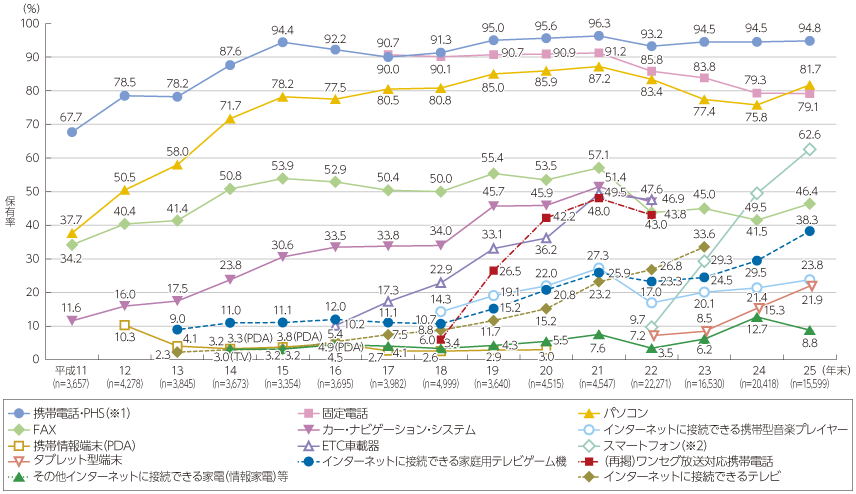
\includegraphics[width=160mm,bb=0 0 856 494]{images/mobiledevicespread.png}
    \caption{情報通信端末世帯保有率の推移(出典:\cite{communicationreport})}
    \label{fig:mobiledevicespread}
  \end{center}
\end{figure}
平成22年には9.7%しかなかったスマートフォンの普及率は、
平成25年には62.6%と急激に成長している。
平成22年から平成25年の3年間で52.9%の伸びを見せており、
これはパソコンの保有率が最も伸びた平成11年から平成14年の
伸び率を大きく上回る数字となっている。
このデータからもスマートフォンの普及は未だかつてないほどの
速度で進んでいることがわかる。

\subsection{モバイルデバイスの用途}
スマートフォンはパソコンの様に多くのことができるが、
文字入力を行う可能性が高いアプリケーションは頻繁に使用されている。
リサーチバンクによるアンケート調査\cite{researchbanksmartphone}
(図:\ref{fig:purpose})によると
\begin{figure}[htbp]
  \begin{center}
    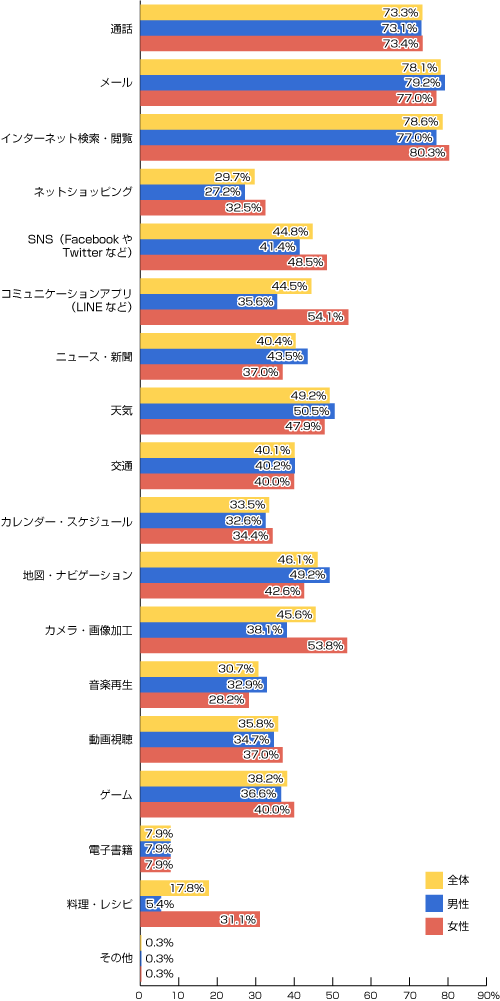
\includegraphics[width=115mm,bb=0 0 500 1001]{images/purpose.png}
    \caption{スマートフォンでどのような機能・アプリを使っているか(出典:\cite{researchbanksmartphone})}
    \label{fig:purpose}
  \end{center}
\end{figure}
メールアプリを使う人が78.1%、SNSアプリを使う人が44.8%、
コミュニケーションアプリを使う人が44.5%となっている。
メールアプリ、コミュニケーションアプリ、SNSアプリはそれぞれ
情報の受信端末としてだけ使う場合には文字入力の必要はないが、
情報を発信しようとする場合には文字入力が必要である。
これら以外の他のアプリにおいても適時文字入力が必要である。
つまりスマートフォンを使うユーザーは文字入力の機会がとても多いことがわかる。
またデバイスが多様化し、文字入力の機会が増えている。
スマートウォッチ(図:\ref{fig:smartwatch})や、
HMDの一つであるGoogle Glass(図:\ref{fig:googleglass})がその例である。
\begin{figure}[htbp]
  \begin{minipage}{0.5\hsize}
    \begin{center}
      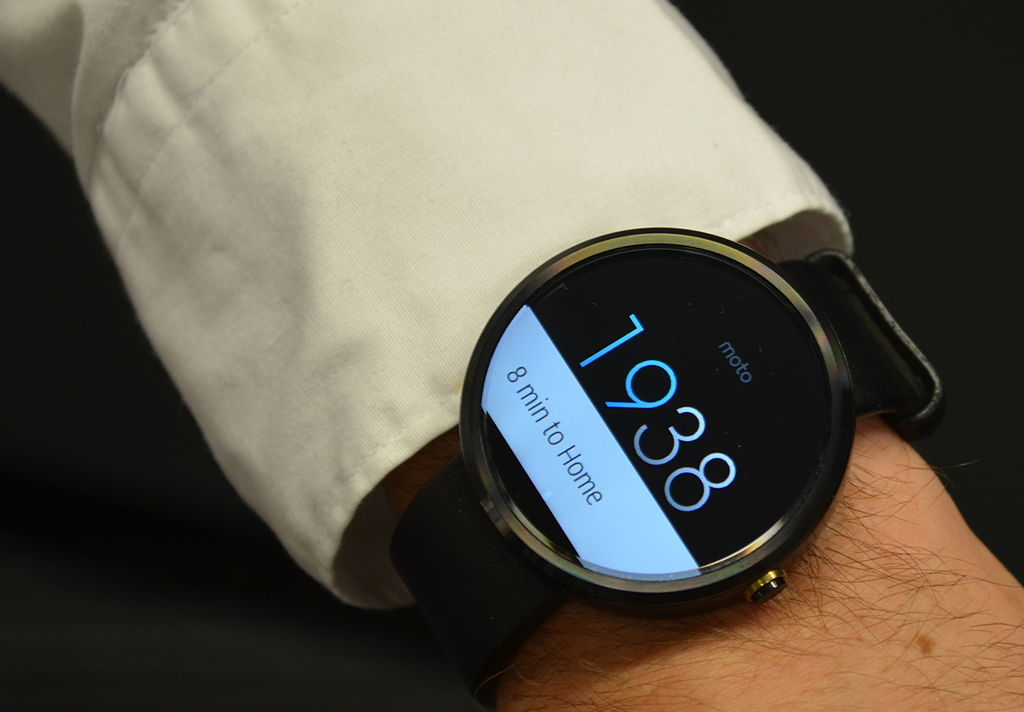
\includegraphics[width=70mm,bb=0 0 246 171]{images/smartwatch.png}
    \end{center}
    \caption{スマートウォッチの例:Android Wearを搭載したMoto360(出典:\cite{smartwatch})}
    \label{fig:smartwatch}
  \end{minipage}
  \begin{minipage}{0.5\hsize}
    \begin{center}
      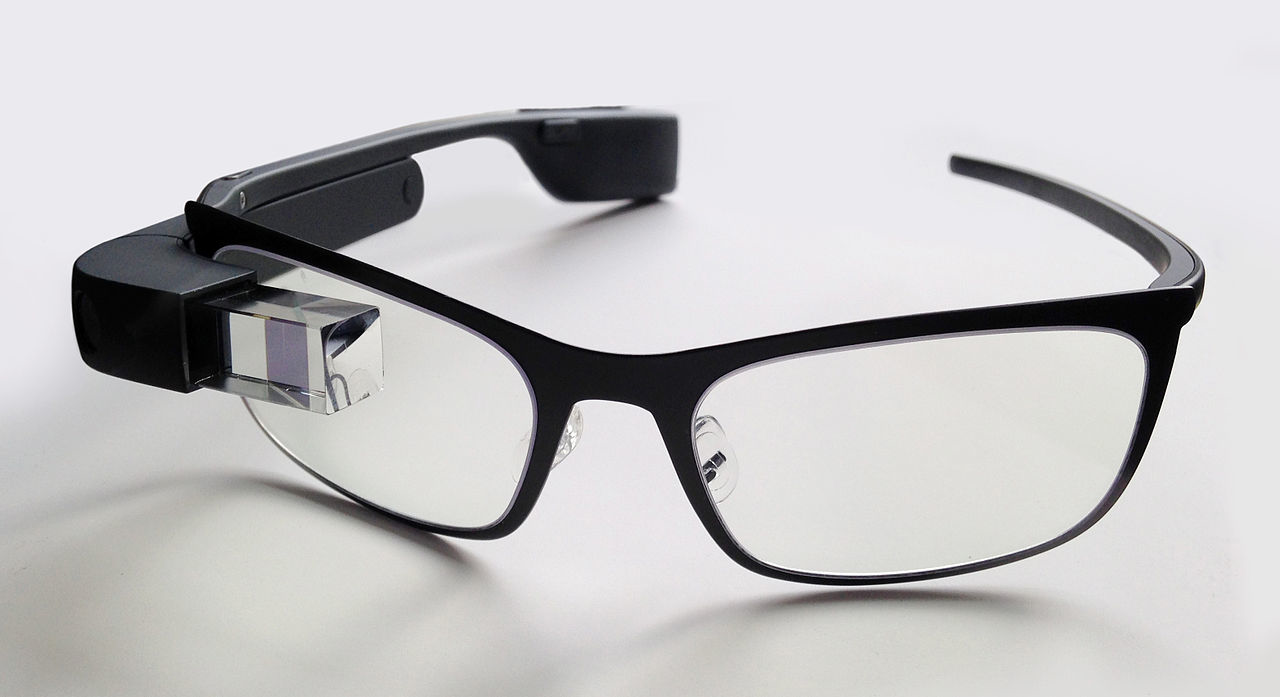
\includegraphics[width=70mm,bb=0 0 1280 697]{images/googleglass.png}
    \end{center}
    \caption{Google glass(出典:\cite{googleglass})}
    \label{fig:googleglass}
  \end{minipage}
\end{figure}
スマートウォッチは既存の時計にモバイルデバイスOSを搭載したもので、
従来の時計であれば文字入力とは無縁であったが、
これを使うことで、文字入力をこのデバイス上でも
行う必要が出てくる。


\section{日本語と英語入力の差異}
日本語と英語では入力にかかるコストが異なる。
qwertyキーボードで日本語を入力する場合、
アルファベットを入力し、それをひらがなに日本語IMEが変換し、
それを漢字やカタカナの混ざった文章に変換するというプロセスをとる。
英語においては入力したアルファベットがそのまま文章となるため、
IMEの必要がなく、ほとんど使われていないのが現状である。

\section{入力システムの変遷}
現在どのようなOSを使用していても必ずIMEアプリケーションは搭載されている。
これらのモバイルデバイスを使う上で日本語の入力は欠かすことができない操作である。
デバイスの性能は携帯電話の頃から劇的に向上している。
パソコンに遜色ないようなメモリやCPUを積んでいるものも多く市販されている。
しかしIMEのシステムに関しては携帯電話の時から大きな変化はない。
日本語IMEにおける内部的なシステムとしては、
連文節変換や予測入力\cite{pobox}の導入がおこなわれ、
広く普及したがまだ改善の余地は多い。
文字入力の方法についても

文字入力にもデバイスに適したよりよいものがある。
文字入力のユーザの体験ももっと向上すべきである。
今回は日本人向けのシステムとして作った。

ユーザにはそれぞれコンテキストがある。
コンテキストによって入力したい単語は推測できるのではないか

\section{問題点と期待}
IMEに関する問題点と期待について述べる。

\subsection{問題点}
楽天リサーチによる「スマートフォンに関する調査」
(出典:\cite{rakutensmartphone})によると、
スマートフォンを使うユーザーが挙げる不満点の中で
最も割合が大きいのが「文字入力がしにくい」ということである。
(出典:\cite{rakutensmartphone})
\begin{figure}[htbp]
  \begin{center}
    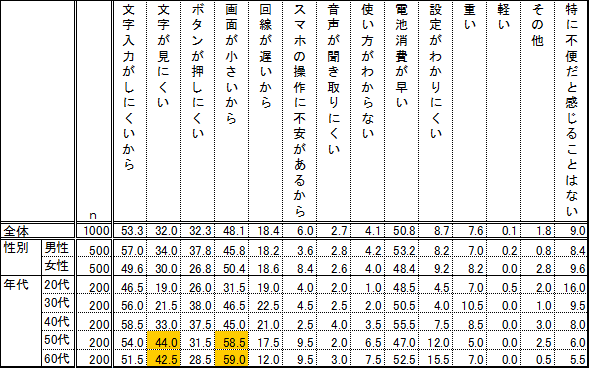
\includegraphics[width=140mm,bb=0 0 589 368]{images/dissatisfaction.png}
    \caption{スマートフォンを利用している際に不便だと感じる点(出典:\cite{rakutensmartphone})}
    \label{fig:dissatisfaction}
  \end{center}
\end{figure}
文字入力がしにくい理由としてはデバイスが携帯電話から
変化しているにもかかわらず、
IMEはほとんど変わっていないためであると考えた。


スマートウォッチやグーグルグラスなどでは文字入力めんどい

\subsection{期待}
最終的には入力したいと思った文字をそのまま
入力できるようなIMEを開発したいと考えている。
その前段階としてコンテキストからユーザーの
入力したい単語を推測し、提示することで
入力のユーザーエクスペリエンスを大幅に向上させるIME
を研究・開発した。
また今回は日本語IMEとして実装したが、
実装されているコンテキスト推薦機能などは
